\documentclass{article}


% if you need to pass options to natbib, use, e.g.:
%     \PassOptionsToPackage{numbers, compress}{natbib}
% before loading neurips_2024


% ready for submission
\usepackage{neurips_2024}


% to compile a preprint version, e.g., for submission to arXiv, add add the
% [preprint] option:
%     \usepackage[preprint]{neurips_2024}


% to compile a camera-ready version, add the [final] option, e.g.:
%     \usepackage[final]{neurips_2024}


% to avoid loading the natbib package, add option nonatbib:
%    \usepackage[nonatbib]{neurips_2024}

\usepackage{graphicx} 
\usepackage[utf8]{inputenc} % allow utf-8 input
\usepackage[T1]{fontenc}    % use 8-bit T1 fonts
\usepackage{hyperref}       % hyperlinks
\usepackage{url}            % simple URL typesetting
\usepackage{booktabs}       % professional-quality tables
\usepackage{amsfonts}       % blackboard math symbols
\usepackage{nicefrac}       % compact symbols for 1/2, etc.
\usepackage{microtype}      % microtypography
\usepackage{xcolor}         % colors

\usepackage{biblatex} %Imports biblatex package
\addbibresource{bibliography.bib} %Import the bibliography file

\title{Semiconductor Layout Design with Large Language Models: Opportunities and Challenges}

\author{%
  Bo Wen\\
  IBM Watson Research Center, \\
  Yorktown Heights, NY, USA \\
  \texttt{bwen@us.ibm.com} \\
  \And
  Xin Zhang\\
  IBM Watson Research Center, \\
  Yorktown Heights, NY, USA \\
  \texttt{xzhang@us.ibm.com} \\
}

\begin{document}

\maketitle

\begin{abstract}
  % Update abstract to reflect the content of the paper
  This paper explores the potential of large language models (LLMs) as a "layout design copilot" in various domains such as semiconductor, IC, and microfluidics. We evaluate the capabilities of LLMs in generating basic elements and combining them into complex designs. Our experiments focus on via connections, microfluidics channel design, and fiducial marker generation. We discuss the opportunities and challenges of using LLMs in layout design, highlighting the importance of providing expert knowledge and context to improve their performance.
\end{abstract}

\section{Introduction}
The semiconductor industry faces numerous challenges in layout design, a critical step in the design and fabrication of integrated circuits (ICs), microfluidic chips, and other electronic devices. One of the most significant challenges is the repetitive nature of drawing similar shapes with minor variations, such as serpentine structures in microfluidic chips with different widths, lengths, number of turns, and tuning radii. \cite{Greengard2024-hx} This repetitive task often violates the "Don't Repeat Yourself" (DRY) principle of software development, leading to inefficiencies and potential inconsistencies in the design process.

Traditional layout design software, which primarily relies on graphical user interfaces (GUIs) rather than scripting-based languages, has struggled to address this issue effectively. However, the advent of Large Language Models (LLMs) presents a new opportunity to revolutionize the layout design process. LLMs have demonstrated remarkable capabilities in understanding natural language instructions, as well as in tasks such as code generation and understanding. By leveraging these capabilities, we can envision a "layout design copilot" that can significantly streamline the design process and improve efficiency.

In this paper, we propose a Neuro-inspired LLM Reasoning Network architecture specifically tailored for adaptive and efficient layout design. Our proposed system allows users to provide natural language instructions to the copilot, describing the desired layout structures and their variations. Additionally, the system can support multimodal inputs, such as sketches, to help communicate the design intent more effectively. The LLM-based copilot then generates code snippets in programming languages like Python, utilizing standard libraries such as gdspy \cite{gdspy} or OASISpy \cite{oasispy} to create GDSII or OASIS files. Furthermore, the copilot can interact with existing layout design software, such as KLayout \cite{klayout}, through APIs or the software's built-in Python environment.

The main contributions of our work are as follows:

1. We introduce a novel Neuro-inspired LLM Reasoning Network architecture that leverages multiple LLMs to generate initial layout design attempts, assess their quality, and reach a consensus on the most promising solutions. This architecture enables more robust and accurate layout generation while mitigating the issue of hallucinations.

2. We demonstrate the effectiveness of our proposed system in the 25 common semiconductor layout design tasks, showcasing its ability to generate accurate and consistent layouts based on natural language instructions and multimodal inputs.

3. We conduct a comprehensive evaluation of our system, comparing its performance against the baseline performance of single-model zero-shot prompting approaches of 5 state-of-the-art LLMs. Our results show significant improvements in terms of zero-shot accuracy and the ability to avoid hallucination-induced mistakes.

The remainder of this paper is structured as follows: Section 2 describes the Neuro-inspired LLM Reasoning Network architecture in detail, highlighting its key components and their interactions. Section 3 presents our experimental setup and the datasets used for evaluation. Section 4 discusses the results of our experiments, comparing the performance of our proposed system against baseline models and state-of-the-art approaches. Section 5 explores potential future directions and applications of our work. Finally, Section 6 concludes the paper, summarizing our findings and contributions.

\section{Neuro-inspired LLM Reasoning Network Architecture}

In this section, we present a novel Neuro-inspired LLM Reasoning Network Architecture designed to enhance the reasoning capabilities of large language models (LLMs) and mitigate the issue of hallucinations in generated outputs. This architecture is particularly well-suited for complex domains such as semiconductor layout design, where the ability to generate accurate and consistent results is critical.

The proposed architecture is inspired by the Brain-like AGI and the Free Energy Principle (FEP) theory. It consists of three main components: Thought Generator Pool, Thought Assessors, and a Steering Subsystem. The Thought Generator Pool is a multi-LLM network that generates initial attempts at a given task by exploring different approaches and perspectives. This multi-LLM approach allows for a more comprehensive exploration of the problem space compared to traditional single-model approaches. It is effectively a Tree-of-Thoughts combined with parallel searching. Because different LLMs have distinct pre-train data and architecture and embedding spaces, this approach can effectively sample diverse solutions from human knowledge space.

The Thought Assessors, also implemented as LLMs, evaluate the outputs generated by the Thought Generator Pool. They analyze the initial attempts, identify consistencies and discrepancies, and reach a consensus on the most promising solutions. By examining the differences between the initial outputs, the Thought Assessors can identify potential hallucinations and mistakes, enabling the system to produce more robust and accurate results.

In the current implementation, a human serves as the Steering Subsystem, coordinating interactions and guiding the overall reasoning process. Additionally, the human performs the active inference function within the Free Energy Principle (FEP) framework. In future work, we aim to develop an automated Steering Subsystem that can distill the system's successes and failures into its knowledge base (a Retrieval-Augmented Generation (RAG) database) to support continual learning.

One of the key advantages of this architecture is its ability to facilitate personal and domain adaptation. By leveraging RAG and continual learning, the system can effectively adapt to specific users' preferences and domain-specific knowledge. This adaptability is particularly valuable in the context of semiconductor layout design, where the ability to tailor the system's outputs to individual designers' needs and domain-specific constraints is essential.

figure 1

Figure 1 illustrates the high-level architecture of the Neuro-inspired LLM Reasoning Network. The Thought Generator, consisting of multiple LLMs, generates initial attempts at the given task. The Thought Assessors evaluate these attempts, identify discrepancies, and reach a consensus on the most promising solutions. The Steering Subsystem coordinates the interactions between the Thought Generator and Thought Assessors, incorporating techniques like RAG and continual learning to enhance the system's adaptability.

figure 2

Figure 2 provides a more detailed view of the interaction between the Thought Generator and Thought Assessors. The Thought Generator produces multiple initial attempts, which are then evaluated by the Thought Assessors. The assessors identify consistencies and discrepancies among the attempts, enabling the detection of potential hallucinations and mistakes. This process allows the system to generate more robust and accurate outputs.

The proposed Neuro-inspired LLM Reasoning Network Architecture offers a significant improvement over traditional single-model approaches in terms of zero-shot accuracy and the ability to avoid hallucination-induced mistakes. By leveraging the power of multiple LLMs and incorporating techniques like RAG and continual learning, this architecture enables more effective reasoning and adaptability in complex domains such as semiconductor layout design.

\section{Baseline LLM Performance in Layout Design}

We evaluated the performance of five large language models (LLMs) - GPT-4o \cite{GPT-4o}, o1-preview \cite{o1-preview}, Claude-3.5-Sonnet \cite{Claude-3.5-Sonnet}, Llama-3.1-70B \cite{Llama-3.1-70B}, and Llama-3.1-405B \cite{Llama-3.1-405B} - on a set of 25 layout design tasks. These tasks were categorized into four groups: Basic Shapes 1, Basic Shapes 2, Advanced Shapes, and Complex Structures. Figure \ref{fig:baseline-llm-performance} presents a summary of the LLMs' performance across the task categories.

\begin{figure}[h]
  \centering
  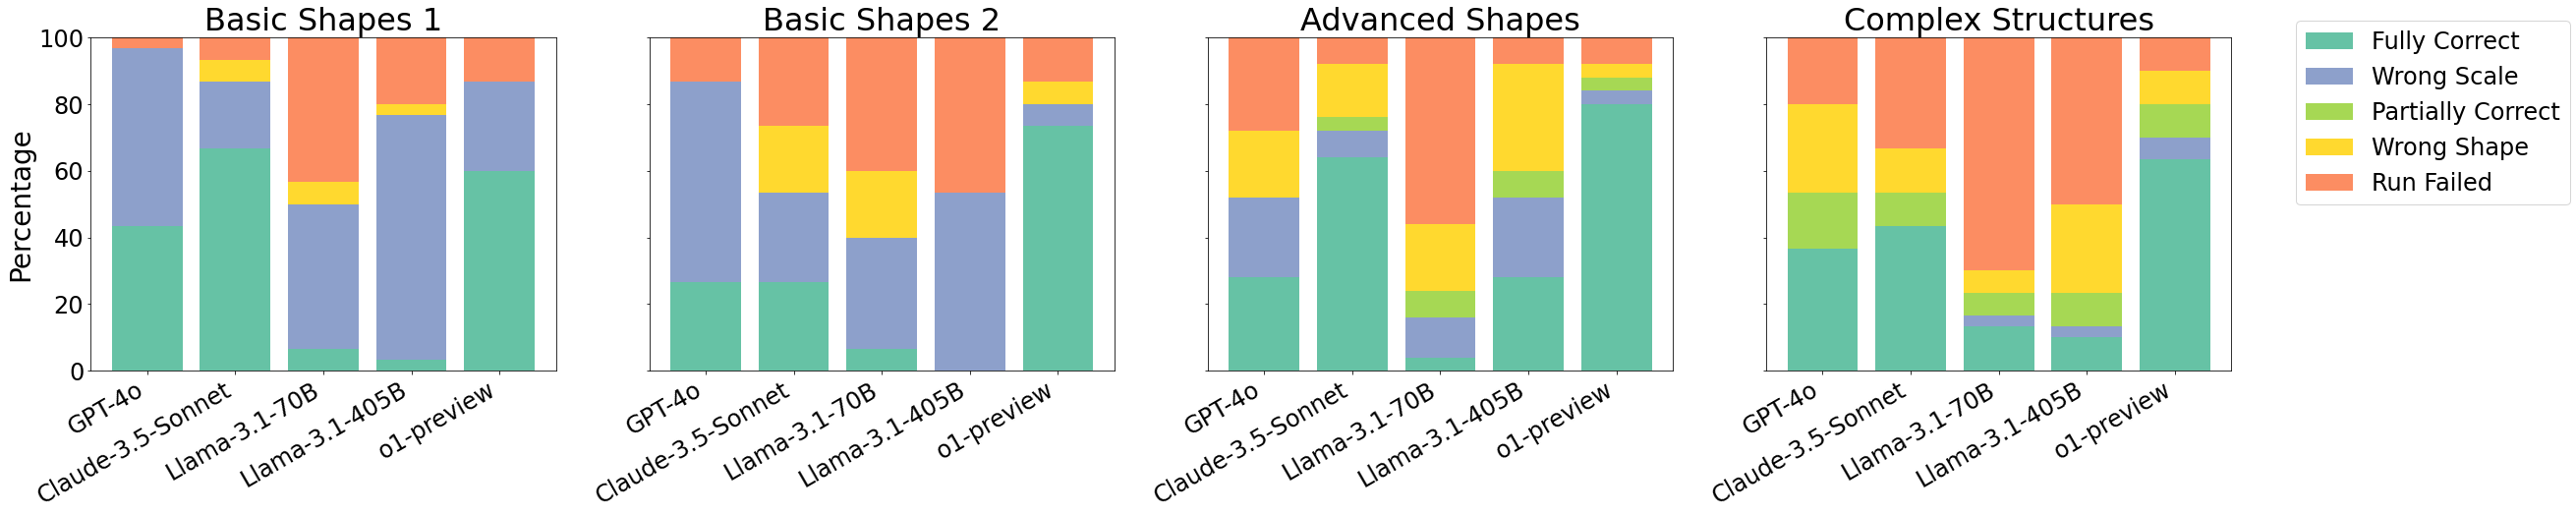
\includegraphics[width=\textwidth]{baseline-llm-performance.png}
  \caption{Baseline LLM Performance on Layout Design Tasks}
  \label{fig:baseline-llm-performance}
\end{figure}

The results reveal several common mistakes and limitations of standalone LLMs in handling layout design tasks:

\begin{enumerate}
  \item \textbf{Incorrect scaling}: Many LLMs struggled with correctly scaling the shapes according to the specified units. The default unit in the gdspy library is micrometers, but most of our basic shape requests were in millimeters. LLMs needed to explicitly scale the lengths by 1000 to obtain the correct output. Some LLMs made incorrect assumptions about the default unit, leading to scaling errors.
  
  \item \textbf{Partial correctness}: In more complex tasks, LLMs often generated partially correct layouts with mistakes in the relative positioning of shapes. For example, in the ViaConnection task, which involved specific location requirements, only o1-preview achieved a fully correct result. The other LLMs produced partially correct outputs with counts: GPT-4o (2), Claude-3.5-Sonnet (2), Llama-3.1-70B (1), and Llama-3.1-405B (3).
  
  \item \textbf{Runtime errors}: Several LLMs generated code that threw exceptions and failed to run. A common error was "AttributeError: module 'gdspy' has no attribute 'LayoutViewer'", which occurred because the LLMs were unaware of the runtime environment. The gdspy version (1.6.3) installed in our Linux VM did not support GUI output, causing this error. Other common errors included AttributeErrors, TypeErrors, and SyntaxErrors, as detailed in the error report (see Appendix).
  
  \item \textbf{Inefficient code}: In some cases, the generated code was inefficient or contained potential issues that caused the program to run very slowly or appear to be stuck. For example, in the DLDChip task, the Llama-3.1-405B model generated code that created a large number of objects and performed numerous boolean operations, leading to high memory usage and extended execution time.
\end{enumerate}

These findings highlight the limitations of standalone LLMs in handling complex layout design tasks. While they perform relatively well on basic shapes, their performance deteriorates as the task complexity increases. The common mistakes and inefficiencies underscore the need for a more advanced approach to tackle these challenges effectively.

A total of 25 examples were generated using ChatGPT-4o, Python code was generated to write a GDSII files for the desired elements, accompanied by human evaluation. In instances where the model did not produce the correct output on the first attempt, a researcher would provide step-by-step guidance until achieving the desired result. However, in the case of generating a serpentine pattern, the model encountered difficulties, likely due to an unfamiliarity with the \texttt{gdspy.FlexPath} function. To address this, an example code was provided to the model, enabling it to 'learn' and successfully generate the correct serpentine sample file.

\subsection{Combining Basic Elements into Complicated Designs}
% Introduction to the three explored use cases
\paragraph{Via connection in semiconductor process}
\paragraph{Microfluidics channel design}


\section{Results and Discussion}
\subsection{Via Connection Experiment}
\subsubsection{Background}
In semiconductor processes, vias are essential for creating electrical connections between different layers of a chip. Proper via placement and connection are crucial for ensuring the functionality and reliability of the integrated circuit. This experiment explores the potential of using large language models (LLMs) to generate layout designs for via connections based on natural language descriptions and color-coded sketches.
\subsubsection{Experimental Setup}
The sketch-to-design approach using LLMs involves providing a natural language description of the desired via connection layout along with a color-coded sketch. The input format consists of a text description specifying the layers, dimensions, positions, and connectivity requirements, as well as a corresponding sketch where each color represents a specific layer (e.g., yellow for via, blue for metal, red for pad). The target output is Python code that generates the GDSII layout based on the provided description and sketch.
\subsubsection{Iterative Testing and Results}
We conducted a series of tests to evaluate the LLM's performance in generating via connection layouts. Figure \ref{fig:via_experiment} presents the sketch input and the corresponding outputs generated by the LLM for each test case.
\begin{figure}[!h]
\centering
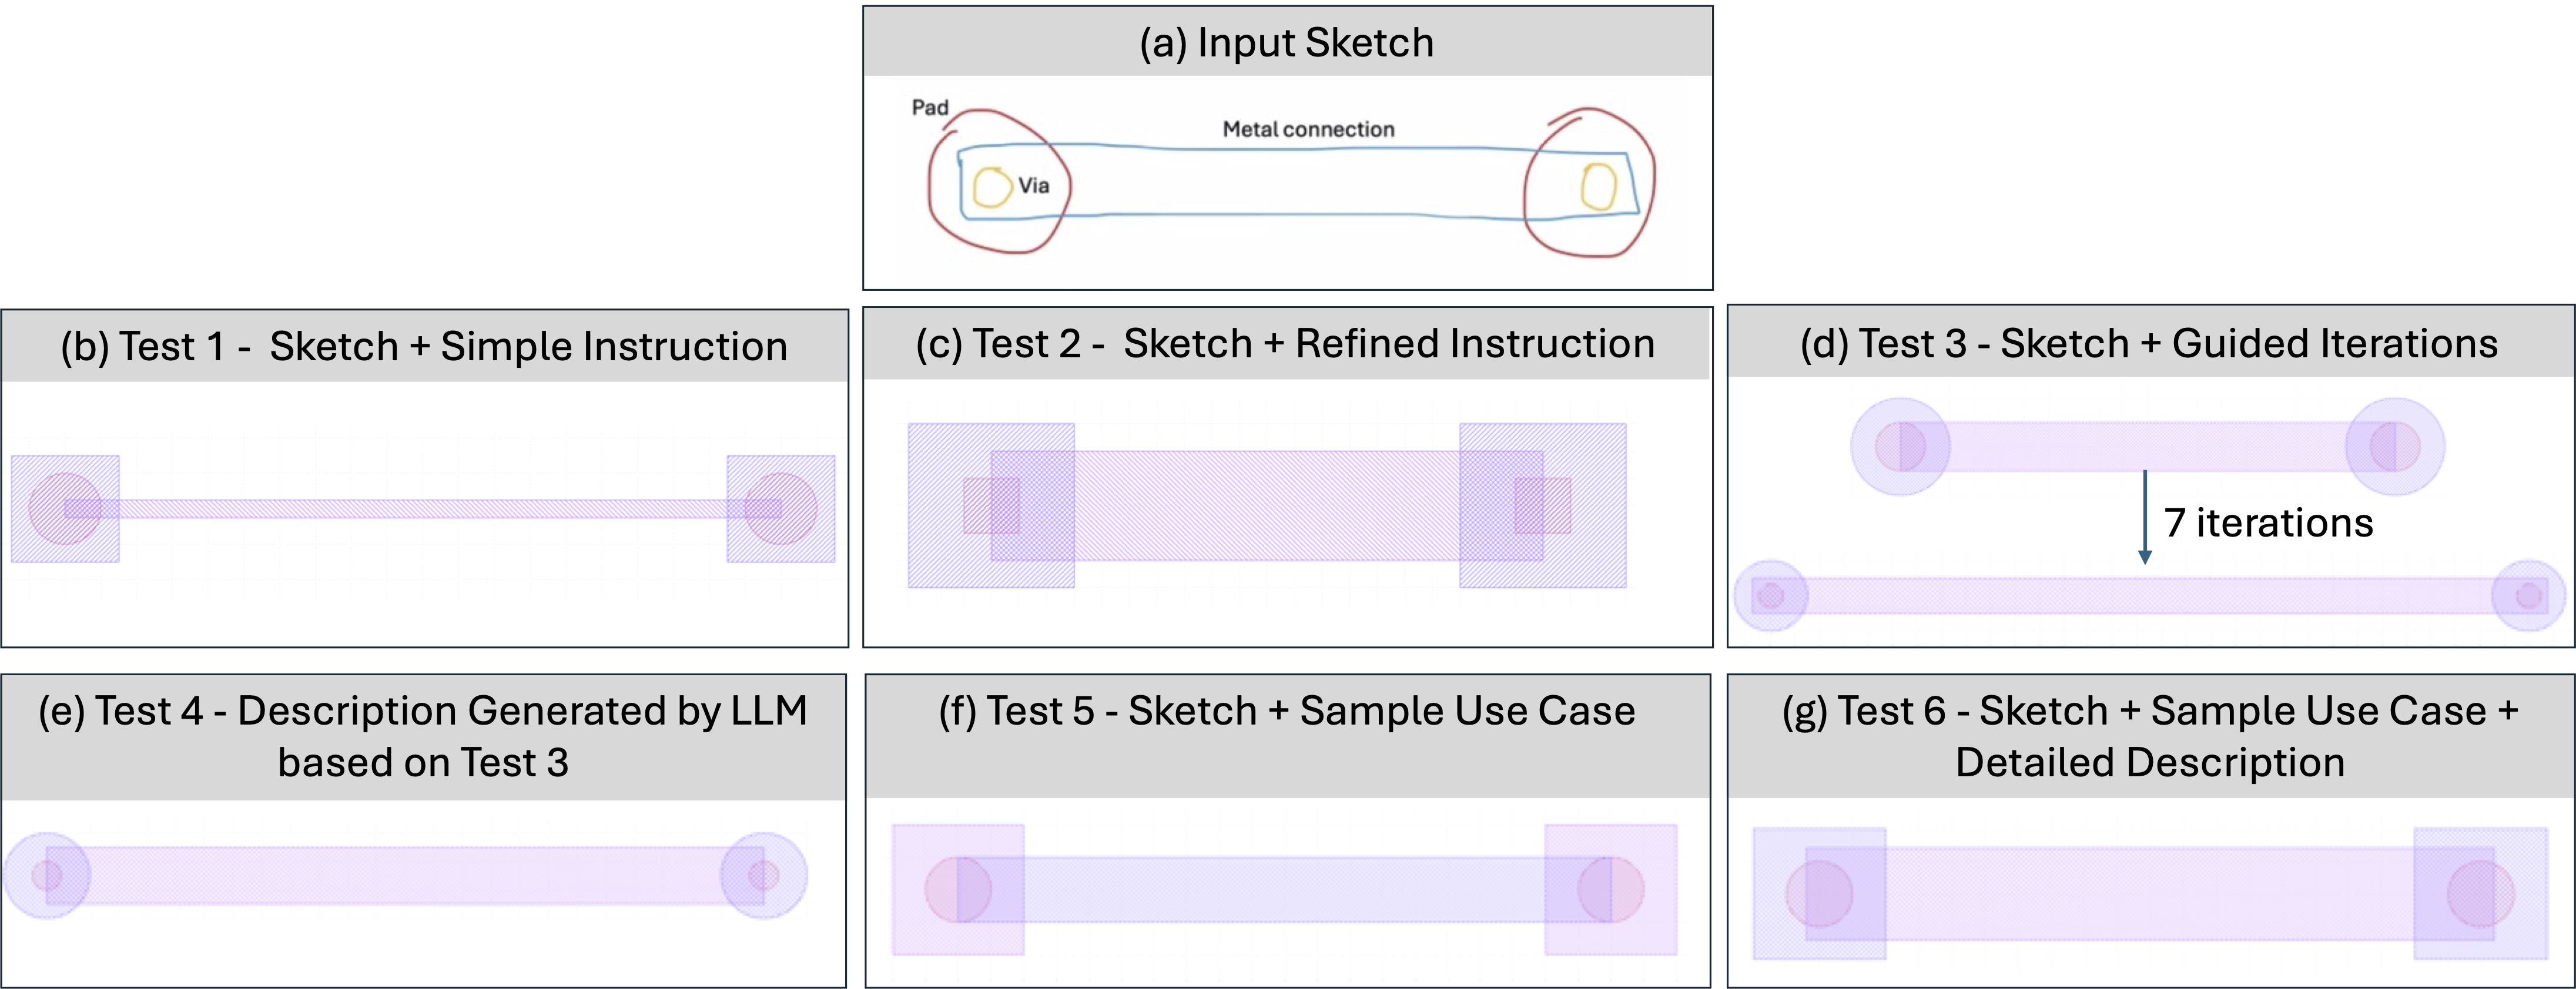
\includegraphics[width=1\linewidth]{Styles/Figure1_v3.png}
\caption{Sketch input and LLM-generated outputs for the via connection experiment. The sketch depicts a desired layout with two vias connected by a metal layer and circular pads on top. The outputs show the progression of the LLM's understanding and refinement of the layout based on iterative feedback and context provided by the user.}
\label{fig:via_experiment}
\end{figure}
In \textbf{Test 1}, we provided a basic sketch (Figure ~\ref{fig:via_experiment}(a)) along with a simple instructions to inform it each color represented a different layer. The LLM generated code based on this initial description; however, the output presented several issues, including incorrect dimensions for various elements and inaccurate layer relationships. \textbf{Test 2} involved refining the description, but limited improvement is observed. 

In \textbf{Test 3}, we gave a more detailed description accompanied by the original sketch. We proceeded with an iterative process, providing the LLM with feedback and screenshots of the GDSII file generated from its code. After seven iterations, the LLM successfully produced the correct layout. \textbf{Test 4} aimed to reproduce the best output from the previous test. We requested the LLM to create a detailed prompt based on the successful result from Test 3 and used this prompt to attempt to generate the correct output again. However, this approach proved ineffective, indicating that relying solely on an LLM-generated prompt to reproduce a layout was not reliable.

\textbf{Tests 5} and \textbf{6} gradually incorporated more context, such as 3D packaging, Through-Silicon Vias (TSVs), and other domain-specific requirements. However, adding domain knowledge and context did not improve the LLM's performance much, showcasing both its limitations and areas for potential improvement. Experienced engineers and researchers understand that connecting two vias requires using a metal layer wider than the diameter of the via. Moreover, vias should not be placed at the very ends of metal layers; some leeway is typically be left between layers to accommodate potential misalignment.

The experiments demonstrate that LLMs currently lack the domain-specific knowledge possessed by experienced engineers, such as the need for wider metal connections between vias and leeway for misalignment. Despite incorporating more context and domain requirements in\textbf{Tests 5} and \textbf{6}, improvements were minimal, highlighting the gap in the LLM's understanding. Future development should focus on embedding domain-specific rules and enhancing consistency and reproducibility.



\subsubsection{Lessons Learned}
The via connection experiment revealed several key findings:
\begin{itemize}
\item Clear, detailed, and context-rich input is essential for LLMs to generate accurate layout designs.
\item Iterative refinement and user feedback play a crucial role in guiding the LLM towards the desired output.
\item LLMs have limitations in understanding domain-specific requirements and constraints without explicit guidance.
\end{itemize}
\subsubsection{Potential Improvements and Future Work}
To enhance the sketch-to-design approach for via connections, we propose incorporating domain-specific knowledge and design rules into the LLM prompts. This can be achieved by providing a comprehensive set of guidelines and constraints as part of the input description. Additionally, future experiments should focus on validating the effectiveness of the improved approach and exploring its applicability to more complex scenarios.

\subsection{General Discussion}
% The importance of spatial thinking, imagination, and understanding of physics for LLMs
% Need for providing use case requirements and expert knowledge as context to LLMs

\section{Conclusion and Future Work}
% Recap the main findings and insights
% Discuss the potential of LLMs in layout design and the challenges to overcome
% Outline future research directions:
%   - Dealing with more complicated designs
%   - Creating a benchmark to test LLM capabilities in layout design tasks
% Final thoughts on the role of LLMs as a "layout design copilot"
agent \cite{Ho2024-cd}
other domains, like mechanics, architecture (3d virtual space \cite{Sasazawa2024-wf})

\printbibliography %Prints bibliography

\end{document}